\chapter{Аналитический раздел}
Архитектура компьютерной сети - это набор уровней и протоколов, 
определяющих принципы построения и функционирования сети. Она позволяет 
различному аппратному и программному обеспечению взаимодействовать 
друг с другом.\cite{kurouz_book} Основными принципами, заложенными в архитектуру компьютерной сети, 
являются:
\begin{itemize}
	\item принцип абстракции - любой уровень должен предоставлять сервисы вышестоящим уровням, скрывая от них детали реализации;
	\item принцип взаимодействия объектов - взаимодействие объектов, находящихся на одном уровне, производится посредством протоколов; 
	\item принцип интерфейса - взаимодействие между соседними уровнями реализуется с помощью интерфейсов.   
\end{itemize}

Одной из моделей архитектуры компьютерной сети является модель TCP/IP. 
Она регламентирует необходимые уровни и протоколы. 
В рамках модели TCP/IP, сокет определяется как конечная точка взаимодействия, 
и в тоже время сокет является интерфейсом, 
который создает уровень абстракции между приложением и сетью. 
Он позволяет процессам использовать стандартные вызовы для обмена данными, 
скрывая детали реализация архитектуры компьютерной сети. 
Таким образом, сокет является элементом архитектуры компьютерной сети.
\section{Анализ сокетов}
В операционной системе Linux сокеты представлены в виде файлового дескриптора. 
Для создания используется системный вызов socket(), 
который принимает три параметра домен, тип и протокол.\cite{man}
Домен определяет пространство адресов,
тип задаёт семантику передачи данных, а протокол конкретизирует используемое
множество сетевых протоколов.
\par
Основными доменами для взаимодействия по сети являются 
AF\_INET для поддержки пространства адресов IPv4 
и AF\_INET6 для поддержки пространства адресов IPv6. 
\par
Основным типами для передачи данных являются SOCK\_STREAM, 
который обеспечивает последовательную, надежную, двустороннюю связь на основе TCP.
и SOCK\_DGRAM, который обеспечивает ненадежную передачу сообщений фиксированной длины на основе UDP.
\par
Стоит отметить, что важным свойством сокета является дуплексная связь - это означает, 
что и процесс сервер, и процесс клиент могут использовать, сокет как для получения данных, так и для их отправки.

\begin{figure}[H]
	\center{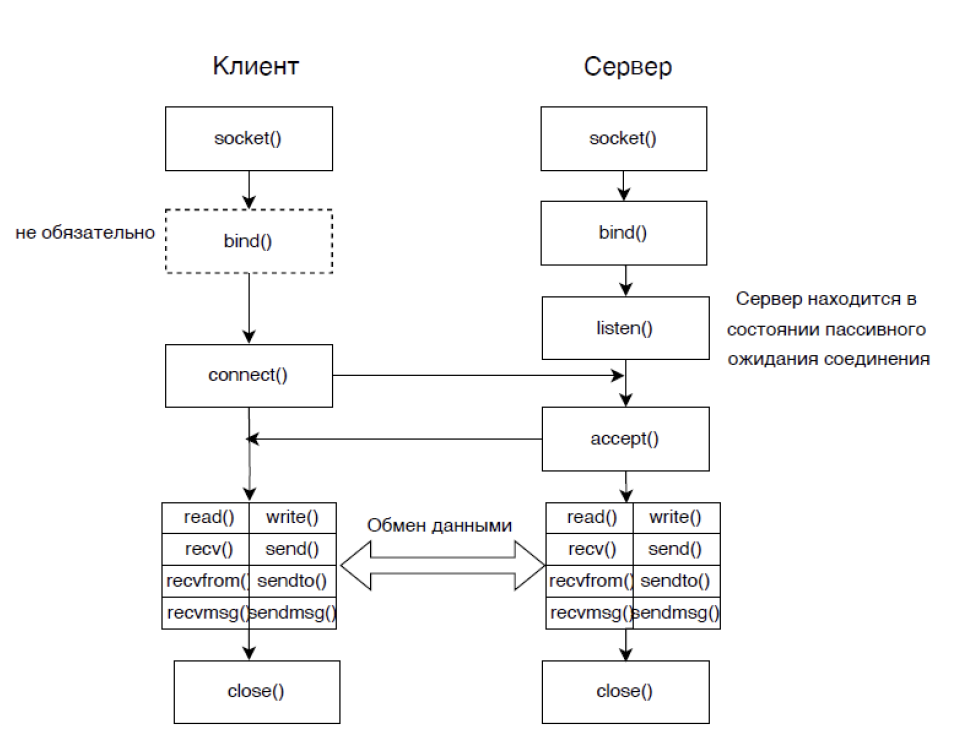
\includegraphics[height=0.82\textheight,width=0.8\textwidth,keepaspectratio]{inc/img/sockets.png}}
	\caption{Схема взаимодействия на сокетах}
	\label{fig:mainAlgo}
\end{figure}

\section{Анализ основных протоколов}
Протокол - это правила и соглашения между сущностями 
одного уровня архитектуры компьютерной сети, 
которые определяют формат передачи данных и процедуры, 
необходимые для передачи информации.\cite{tanen_book}
\par
На транспортном уровне модели TCP/IP выделяют два основных протокола TCP и UDP.
TCP (Transmission Control Protocol) - это протокол c установлением соединения, 
обеспечивающий надежный сквозной байтовый поток по ненадежной интерсети.
Здесь надежность означает то, 
что протокол гарантирует достаку данных без ошибок, потерь и дублирования. 
А установление соединения означает то, 
что, перед обменом информацией, необходимо совершить «трёхстороннее рукопожатие»

UDP (User Datagram Protocol) - это ненадежный протокол без установления соединения.
\par 
Протокол прикладного уровня HTTP (HyperText Transfer Protocol), 
используемый для передачи веб-страниц и в большинстве случаев работающий поверх протокола TCP, 
работает по модели запрос-ответ.

Модель запрос-ответ регламентирует взаимодействие между процессом клиентом и процессом сервером. 
Так, основными методами процесса клиента по протоколу HTTP явлются:
\begin{itemize}
	\item GET - получение 
	\item POST - добавление
	\item DELETE - удаление
	\item PATCH - неполное изменение 
	\item PUT - полное идемпотентное изменение
\end{itemize}
А основные состояния, которые процесс сервер возвращает в виде кодов, согласно протоколу HTTP,
являются:
\begin{itemize}
	\item 1xx - информационные
	\item 2xx - успех
	\item 3xx - перенаправление
	\item 4xx - ошибка клиента
	\item 5xx - ошибка сервера
\end{itemize}

\section{Анализ системных вызовов}
Помимо предоставления абстракции конечной точки взаимодействия - сокета,
операционная система Linux поддерживает механизм потоков и мультиплексирования. 

\subsection{Анализ потоков в Linux}
Выделяют следующие типы потоков:
\begin{itemize}
	\item потоки ядра (kernel threads) - создаются внутри ядра
	с помощью kthread\_create().
	Не имеют пользовательского адресного пространства (mm = NULL),
	выполняются исключительно в пространстве ядра,
	которое разделяют со всеми остальными потоками.
	\item пользовательские потоки в модели M:1 - создаются и планируются
	библиотекой в пользовательском пространстве без участия ядра.
	Ядро видит только один поток, а библиотека-менеджер
	самостоятельно распределяет процессорное время.
	Недостаток - блокирующий системный вызов в одном потоке
	блокирует все потоки процесса, так как ядро не различает их; \cite{nptl}
	\item пользовательские потоки в модели 1:1 - каждому пользовательскому потоку
	соответствует ровно один поток ядра.
	В Linux стандартная библиотека glibc реализует данную модель
	через подсистему NPTL (Native POSIX Threads Library):
	вызов pthread\_create()\cite{man} порождает поток ядра через системный вызов
	clone() с флагами CLONE\_VM, CLONE\_FILES,
	CLONE\_THREAD. \cite{drepper}
	Планирование полностью делегируется планировщику ядра (CFS),
	что устраняет проблему блокировки модели M:1. 
\end{itemize}

Основным свойством потоков является наследование адресного пространства родителя:
для пользовательских потоков - это адресное пространство процесса родителя,
а для потоков ядра - пространство ядра, общее для всех потоков.
Из данного свойства следует необходимость обеспечения синхронизации
доступа к разделяемым ресурсам с помощью примитивов,
таких как мьютексы или семафоры.

\subsection{Анализ мультиплексирования ввода-вывода в Linux}
Мультиплексирование ввода-вывода - это механизм, позволяющий одному потоку
выполнения одновременно отслеживать состояние готовности нескольких файловых
дескрипторов. В контексте веб-сервера это означает возможность обслуживать
множество клиентских соединений без выделения отдельного потока на каждое из них.

В ОС Linux реализованы следующие системные вызовы мультиплексирования:
\begin{itemize}
	\item select() - принимает три множества дескрипторов
	(чтение, запись, исключения), представленных битовыми масками fd\_set.
	Ограничение - максимальный номер дескриптора определяется константой
	FD\_SETSIZE (по умолчанию 1024).
	При каждом вызове ядро линейно проверяет все дескрипторы в множестве,
	что даёт сложность $O(n)$, где $n$ - максимальный номер дескриптора; \cite{mike_book}
	\item poll() - принимает массив структур pollfd,
	каждая из которых содержит дескриптор, запрашиваемые и возвращённые события.
	Снимает ограничение FD\_SETSIZE,
	однако сложность остаётся $O(n)$, так как ядро проверяет весь массив;
	\item epoll - подсистема, состоящая из трёх системных вызовов:
	epoll\_create() создаёт экземпляр epoll,
	epoll\_ctl() регистрирует или удаляет дескрипторы,
	epoll\_wait() блокирует поток до наступления события.
	В отличие от select() и poll(),
	ядро поддерживает внутреннюю структуру данных
	и возвращает только готовые дескрипторы,
	что даёт сложность $O(k)$, где $k$ - количество готовых дескрипторов. \cite{mike_book}
\end{itemize}

При регистрации дескриптора через epoll\_ctl()
указываются флаги событий, которые необходимо отслеживать:
\begin{itemize}
	\item EPOLLIN - дескриптор готов к чтению;
	\item EPOLLOUT - дескриптор готов к записи;
	\item EPOLLERR - произошла ошибка на дескрипторе;
	\item EPOLLHUP - разрыв соединения;
	\item EPOLLRDHUP - удалённая сторона закрыла соединение или запись;
	\item EPOLLONESHOT - после срабатывания дескриптор деактивируется
	до повторной регистрации через epoll\_ctl().
\end{itemize}

epoll поддерживает два режима срабатывания:
\begin{itemize}
	\item level-triggered (по умолчанию) - событие генерируется,
	пока дескриптор остаётся в состоянии готовности;
	\item edge-triggered (флаг - EPOLLET) - событие генерируется
	однократно при переходе дескриптора в состояние готовности.
\end{itemize}

Таким образом, для реализации многопоточного веб-сервера
epoll является предпочтительным механизмом мультиплексирования,
поскольку его производительность в теории не деградирует
с ростом числа одновременных соединений.